% CAP description for Tabbed Pane
A \bxname{tabbed pane} is a container that allows you to switch between multiple groups of components within a single area.



\begin{figure}
\begin{center}
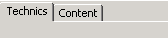
\includegraphics{PS/Tab}
\caption{Tabbed Pane}
\label{tabbedpane}
\end{center}
\end{figure}

\textbf{Mapping tabbed panes}

In the \gdomm{}, a tabbed pane to be mapped looks like this:

\begin{figure}
\begin{center}
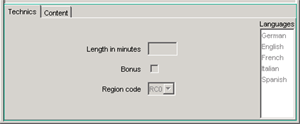
\includegraphics{PS/Maptab}
\caption{Tabbed Pane}
\label{maptab}
\end{center}
\end{figure}
